\section{Drugi algorytm (\textbf{Metoda18})}
\textbf{Metoda18} to integracja \textbf{wzmacniania gradientowego (Gradient Boosting)} i \textbf{CatBoost}, wzbogacona o meta-model w postaci \textbf{regresji logistycznej}. Algorytm jest wynikiem połączenia pomysłów pochodzących z \textbf{Metody12} oraz \textbf{Metody13}. \textbf{Metoda13} została zaimplementowana przy użyciu \textbf{warstwowego łączenia modeli}, gdzie \textbf{Gradient Boosting}, \textbf{XGBoost} i \textbf{losowy las (RandomForestClassifier)} były łączone przy użyciu \textbf{regresji logistycznej} jako meta-modelu. \textbf{Metoda12} natomiast wykorzystywała wyłącznie \textbf{CatBoost}, co pokazało jego dużą skuteczność w pracy z danymi kategorialnymi i nierównomiernymi, co również wpłynęło na wybór tego modelu w obecnym podejściu.

\textbf{Metoda18} czerpie z \textbf{Metody13} mechanizm \textbf{warstwowego łączenia modeli}, jednak zamiast wielu modeli bazowych, opiera się na dwóch potężnych algorytmach: \textbf{Gradient Boosting} i \textbf{CatBoost}. Wybór tych modeli wynika z ich zdolności do radzenia sobie z różnymi typami danych i ich nierównowagą. \textbf{Regresja logistyczna} jako meta-model umożliwia skuteczną integrację wyników, co zostało wcześniej zademonstrowane w \textbf{Metodzie13}.

\subsection{Wejściowe parametry}
Metoda \textbf{train\_run18} przyjmuje następujące parametry wejściowe:

\begin{enumerate}
	\def\labelenumi{\arabic{enumi}.}
	\item
	      \textbf{X\_train}: Macierz danych treningowych, gdzie każdy wiersz to jedna próbka, a kolumny to cechy. Rozmiar: n - liczba próbek, m - liczba cech.
	\item
	      \textbf{y\_train}: Wektor etykiet dla danych treningowych. Rozmiar: n, gdzie n - liczba próbek w danych treningowych.
	\item
	      \textbf{X\_test}: Macierz danych testowych, analogiczna do \textbf{X\_train}, używana do oceny modelu.
	\item
	      \textbf{y\_test}: Wektor etykiet testowych, odpowiadający danym testowym.
\end{enumerate}

\subsection{Wyjściowe parametry}
Metoda zwraca następujące elementy:

\begin{enumerate}
	\def\labelenumi{\arabic{enumi}.}
	\item
	      \textbf{meta\_model}: Meta-model (\textbf{regresja logistyczna}) wytrenowany na danych pochodzących z predykcji modeli \textbf{wzmacniania gradientowego} i \textbf{CatBoost}.
	\item
	      \textbf{meta\_features\_test}: Macierz meta-cech, zbudowana na podstawie predykcji modeli bazowych dla danych testowych.
	\item
	      \textbf{y\_test}: Wektor etykiet testowych, identyczny z wejściowym \textbf{y\_test}.
\end{enumerate}

\subsection{Algorytm}
\begin{enumerate}
	\def\labelenumi{\arabic{enumi}.}
	\item
	      Trenowanie modeli bazowych:
	      \begin{itemize}
		      \item
		            \textbf{Gradient Boosting}: Inicjalizuje się \textbf{GradientBoostingClassifier} z liczbą 100 estymatorów i zachowaniem losowości (\textbf{random\_state=42}). Następnie przeprowadza się trenowanie na \textbf{X\_train} i \textbf{y\_train}.
		      \item
		            \textbf{CatBoost}: Inicjalizuje się \textbf{CatBoostClassifier} z ustawionymi 100 iteracjami, kontrolowaną losowością (\textbf{random\_state=42}) i wyłączonymi komunikatami. Następnie przeprowadza się trenowanie na \textbf{X\_train} i \textbf{y\_train}.
	      \end{itemize}
	\item
	      Generowanie predykcji dla danych treningowych:
	      \begin{itemize}
		      \item
		            Oblicza się prawdopodobieństwa pozytywnej etykiety: \textbf{gb\_preds\_train} (predykcje \textbf{wzmacniania gradientowego}) oraz \textbf{cat\_preds\_train} (predykcje \textbf{CatBoost}).
		      \item
		            Tworzy się macierz meta-cech z \textbf{gb\_preds} i \textbf{cat\_preds} jako kolumnami.
	      \end{itemize}
	\item
	      Trenowanie meta-modelu:
	      \begin{itemize}
		      \item
		            Przeprowadza się trenowanie \textbf{regresji logistycznej} na \textbf{meta\_features\_train} i \textbf{y\_train}. \textbf{Regresja logistyczna} łączy predykcje modeli bazowych.
	      \end{itemize}
	\item
	      Generowanie predykcji dla danych testowych:
	      \begin{itemize}
		      \item
		            Oblicza się prawdopodobieństwa klasy pozytywnej: \textbf{gb\_preds\_test} (predykcje \textbf{Gradient Boosting}) oraz \textbf{cat\_preds\_test} (predykcje \textbf{CatBoost}).
		      \item
		            Tworzy się macierz meta-cech dla danych testowych, analogicznie do treningowych.
	      \end{itemize}
	\item
	      Zwracanie wyników: Zwraca się wytrenowany \textbf{meta\_model}, \textbf{meta\_features\_test} i \textbf{y\_test}.
\end{enumerate}

Szczegółowy schemat \textbf{metoda18} przedstawiono na diagramie \ref{fig:diagram_metoda18}. Pomarańczowe prostokąty odpowiadają pomysłom, które opierały się na podejściu z \textbf{metoda13}. Natomiast zielone prostokąty podkreślają zamysł, którym inspirowałem się z \textbf{metoda12}.

\begin{figure}[H]
	\centering
	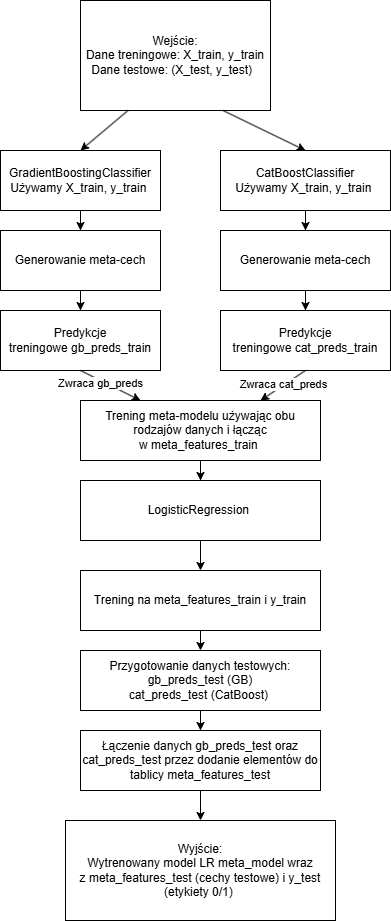
\includegraphics[width=0.7\textwidth]{img/diagrams/metoda18.drawio.png}
	\caption{Schemat metody 18.}
	\label{fig:diagram_metoda18}
\end{figure}

\subsection{Właściwości analityczne}
\begin{enumerate}
	\def\labelenumi{\arabic{enumi}.}
	\item
	      \textbf{Efektywność}:
	      \begin{itemize}
		      \item
		            Kombinacja \textbf{wzmacnianie gradientowe} i \textbf{CatBoost} pozwala na efektywne uchwycenie zarówno liniowych, jak i nieliniowych zależności w danych.
		      \item
		            Meta-model optymalizuje końcowe wyniki poprzez fuzję predykcji z modeli bazowych.
	      \end{itemize}
	\item
	      \textbf{Elastyczność}: Metoda może być zastosowana w różnych problemach klasyfikacyjnych, szczególnie w przypadkach, gdzie różne modele bazowe wykazują różne mocne strony.
	\item
	      \textbf{Stabilność}: Meta-model działa jako mechanizm konsolidujący, zmniejszając wariancję predykcji i poprawiając stabilność wyników.
	\item
	      \textbf{Złożoność obliczeniowa}:
	      \begin{itemize}
		      \item
		            Zarówno \textbf{wzmacnianie gradientowe}, jak i \textbf{CatBoost} mają złożoność liniową względem liczby próbek i estymatorów, co pozwala na efektywne przetwarzanie dużych zbiorów danych.
		      \item
		            Dodanie meta-modelu nieznacznie zwiększa złożoność, ale poprawia jakość wyników.
	      \end{itemize}
	\item
	      \textbf{Wydajność}: \textbf{CatBoost} jest zoptymalizowany pod kątem szybkiego trenowania, a \textbf{wzmacnianie gradientowe} zapewnia interpretowalność wyników. Kombinacja tych dwóch modeli z meta-modelem znacząco poprawia skuteczność klasyfikacji.
\end{enumerate}